% TODO put all names of steps according to \methontology into \emph
% TODO ontology - naming conventions
% TODO mention - this chapter does not cover the ontology development process as it was done; instead, it presents the completed documents that were created in that processs.
% TODO mention second paper about methontology (the one that describes all artefacts created when building the chemical ontology)

% TODO check if the things mentioned here are properly covered in the chapters referred

% TODO rename: belongsToWeatherReport -> belongsToReport

% TODO elaborate steps more?

% TODO reference paper: Building legal ontologies with METHONTOLOGY and WebODE

The previous chapters covered all aspects that have to be analyzed in order to build a completely new ontology from scratch: Chapter \ref{ch:weather_data} discussed all details about weather data necessary for the \thinkhome weather ontology, what data will be used and where to obain it. Chapter \ref{ch:existing_work} gave an overview over existing work regarding ontologies in the domain of weather data. As none of the existing ontologies fit the needs of an ontology for \thinkhome, chapter  \ref{ch:development_approaches} analyzed some of the most popular approaches for building ontologies from scratch. Among those \methontology was identified as the best suitable approach. % TODO citation for methontology?

Based on these findings, this chapter describes the process of building the \thinkhome weather ontology in detail. The structure follows the steps in the ontology development process introduced by \methontology.

\section{Specification}
\label{sec:ontology_specification}

Specification, the first step proposed by \methontology, aims at creating an ontology specification document using natural language. That document must include at least the intended purpose of the ontology, the level of 
formality and the ontology's scope.

% TODO ensure there are no problematic page breaks inside this box (e.g. between the headline 'Scope:' and the first bullet point)
\begin{mdframed}
\setlength{\parindent}{0pt}
\MakeUppercase{\textbf{Ontology requirements specification document}}

\vspace{.5cm}

\textbf{Domain}: Weather data

\vspace{.2cm}

\textbf{Date}: 2012 % TODO

\vspace{.2cm}

\textbf{Purpose}: The ontology shall cover data about weather phenomena occurring at a certain location somewhere on Earth between the present and 24 hours in the future. Weather data will be aquired from both internet services as well as from weather sensors mounted to a building. This weather data will enable the \textit{ThinkHome} system to make decisions based on current and future weather conditions.

\vspace{.2cm}

\textbf{Level of formality}: semi-informal % TODO citations for uschold & gruninger, 1996; uschuld & king (enterprise ontology)

\vspace{.2cm}

\textbf{Scope}:

\begin{itemize}
  \item \emph{Weather phenomenon}: Represents a certain weather element. Relevant weather elements are temperature, humidity, dew point, wind speed and direction, precipitation intensity and probability, atmospheric pressure, cloud cover, sun radiation, and the sun's position.

  \item \emph{Weather condition}: Overall state of the weather: sun, light clouds, partly cloudy, cloudy, fog, rain, snow, sleet, thunder.
  \item \emph{Weather state}: Summarizes all weather phenomena for a certain time. 
  \item \emph{Weather report}: Summarizes all data aquired at a certain time about the current weather or the weather some time in the future. Exactly one weather state is linked to each weather report.
  \item \emph{Weather report source}: Source where the data belonging to a weather report has been obtained from (either a internet weather service or a local weather sensor).
\end{itemize}

\vspace{.2cm}

\textbf{Sources of knowledge}: % TODO reference more literature (e.g. for types of twilight)
\begin{itemize}
  \item Weather data that is available from internet services.
  \item Weather data that is available from local weather sensors.
  \item Existing ontologies that cover the domain of weather data.
  \item Information about weather in general, e.g. the Glossary of Meteorology by the American Meteorological Society. % TODO citation, more literature
\end{itemize}

% TODO reference previous chapter
\textbf{Competency questions}:
\begin{itemize}
  \item What is the current weather situation?
  \item What will the weather situation be in one hour, in two hours, …, in 24 hours?
  \item What is the current temperature, humidity, wind speed, …?
  \item What will be the temperature, humidity, wind speed, … in one hour, in two hours, …, in 24 hours?
  \item What will be the minimum temperature, humidity, … over the next 24 hours? What about maximum values?
  \item Will the weather change? Will the temperature, humidity, … rise or fall?
  \item Does it rain? Will it rain in the next hours? Will it rain today?
  \item Will there be sunshine today? 
  \item Do we need to irrigate the garden?
  \item Will there be severe weather?
  \item Will temperature drop/stay below $0^\circ C$?
  \item When can we open windows and when do we have to keep them shut?
  \item When do we need sun protection?
  \item When will it outside be colder than inside the house? When will it be warmer?
\end{itemize}

\end{mdframed}

\vspace{.5cm}

In the following sections, the \thinkhomeweather ontology is built in a way to meet all above requirements. Section \ref{ch:ontology_evaluation} evaluates if the ontology that has been developed fits the specification and what the ontology's shortcomings are.

\section{Knowledge Aquisition}

The step of knowledge aquisition was already described in the previous chapters \ref{ch:existing_work} and \ref{ch:weather_data}. These chapters disussed in detail:

\begin{itemize}
  \item Which weather data are relevant for \thinkhome?
  \item Which weather data are available from sensors and internet services? How can this data be acquired?
  \item Which data do not have any use for \thinkhomeweather due to being too complicated or because they cannot be processed in an ontology in a useful way?
  \item What knowledge about weather in general is required to build an appropriate ontology? % TODO check if this is available in the previous chapters
\end{itemize}

\section{Conceptualization}

In the conceptualization step, the domain knowledge is structured in a conceptial model that describes the problem and its solution in terms of the domain vocabulary identified in the specification step. At first, a complete Glossary of Terms is built that covers all concepts, instances, attributes and binary relations.

\subsection{Glossary of Terms}

% TODO mention: in alphabetical order
% TODO repeat header on every page?
% TODO references between glossary items; e.g. from 'civil twilight' to 'twilight'
% TODO add sub-concepts for weather state
% TODO add type column
% TODO add binary relations
\begin{longtable}{|p{0.25\textwidth}|p{0.7\textwidth}|}
  \hline
  \textbf{Name} & \textbf{Description} \\
  \hline\hline
  Above room temperature & \\
  \hline
  Altitude & \\
  \hline
  Astronomical twilight & \\
  \hline
  Atmospheric pressure & \\
  \hline
  Below room temperature & \\
  \hline
  Calm & \\
  \hline
  Civil twilight & \\
  \hline
  Clear sky & \\
  \hline
  Cloud & \\
  \hline
  Cloud cover & \\
  \hline
  Cold & \\
  \hline
  Condition weather state & \\
  \hline
  Current weather report & \\
  \hline
  Current weather report from sensor & \\
  \hline
  Current weather report from service & \\
  \hline
  Day & \\
  \hline
  Dew point & \\
  \hline
  Directional wind & \\
  \hline
  Dry & \\
  \hline
  East wind & \\
  \hline
  End time & \\
  \hline
  Extremely heavy rain & \\
  \hline
  Fog & \\
  \hline
  Forecast weather report & \\
  \hline
  Frost & \\
  \hline
  Heat & \\
  \hline
  Heavy rain & \\
  \hline
  High pressure & \\
  \hline
  High radiation & \\
  \hline
  Humidity & \\
  \hline
  Hurricane & \\
  \hline
  Latitude & \\
  \hline
  Light clouds & \\
  \hline
  Light rain & \\
  \hline
  Light wind & \\
  \hline
  Location & \\
  \hline
  Longitude & \\
  \hline
  Long range weather report & \\
  \hline
  Low pressure & \\
  \hline
  Low radiation & \\
  \hline
  Medium radiation & \\
  \hline
  Medium rain & \\
  \hline
  Medium range weather report & \\
  \hline
  Moist & \\
  \hline
  Mostly cloudy & \\
  \hline
  Nautical twilight & \\
  \hline
  Night & \\
  \hline
  No radiation & \\
  \hline
  No rain & \\
  \hline
  Normal humidity & \\
  \hline
  Normal pressure & \\
  \hline
  North wind & \\
  \hline
  Observation time & \\
  \hline
  Overcast & \\
  \hline
  Partly cloudy & \\
  \hline
  Precipitation & \\
  \hline
  Priority & \\
  \hline
  Rain & \\
  \hline
  Room temperature & \\
  \hline
  Sensor source & \\
  \hline
  Service source & \\
  \hline
  Short range weather report & \\
  \hline
  Sleet & \\
  \hline
  Snow & \\
  \hline
  Solar twilight & \\
  \hline
  South wind & \\
  \hline
  Start time & \\
  \hline
  Storm & \\
  \hline
  Strong wind & \\
  \hline
  Sun & \\
  \hline
  Sun from east & \\
  \hline
  Sun from north & \\
  \hline
  Sun from south & \\
  \hline
  Sun from west & \\
  \hline
  Sun position & \\
  \hline
  Sun radiation & \\
  \hline
  Temperature & \\
  \hline
  Thunder & \\
  \hline
  Timed weather report & \\
  \hline
  Tropical storm rain & \\
  \hline
  Unknown cloud cover & \\
  \hline
  Very dry & \\
  \hline
  Very high pressure & \\
  \hline
  Very high radiation & \\
  \hline
  Very low pressure & \\
  \hline
  Very moist & \\
  \hline
  Weather condition & \\
  \hline
  Weather phenomenon & \\
  \hline
  Weather report & \\
  \hline
  Weather report from sensor & \\
  \hline
  Weather report from service & \\
  \hline
  Weather report source & \\
  \hline
  Weather state & \\
  \hline
  West wind & \\
  \hline
  Wind & \\
  \hline
\end{longtable}

\subsection{Concept-classification trees}
\label{sec:concept_classification_trees}

All concepts from the Glossary of Terms can be organized into five categories. Each of these categories has one root concept. These are \emph{Weather condition}, \emph{Weather phenomenon}, \emph{Weather report}, \emph{Weather report source} and \emph{Weather state}. All other concepts are sub-concepts of one of these five root concepts. The trees resulting from the structure are presented below.

\subsubsection{Weather condition}

A \emph{Weather condition} represents a simple verbal description of the weather state at a certain time. As it does not have any sub-concepts, the diagram showing this classification tree looks rather simple:

\begin{center}
  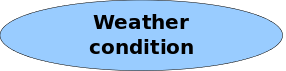
\includegraphics[scale=.3]{figures/diagrams/weather-condition.png}
\end{center}

\subsubsection{Weather phenomenon}

A \emph{Weather phenomenon} represents a certain weather element, e.g. temperature or humidity. Every specific weather element is a sub-concept of \emph{Weather phenomenon}. Hence, this tree evolves:

\begin{center}
  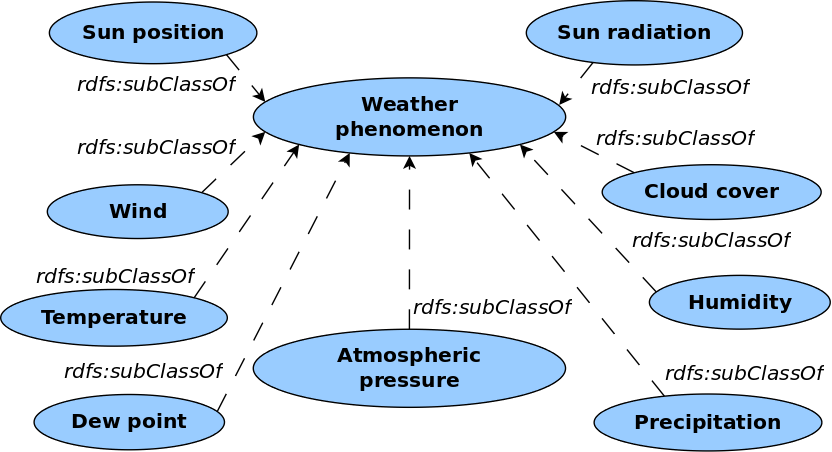
\includegraphics[scale=.3]{figures/diagrams/weather-phenomenon.png}
\end{center}

Every of these sub-concepts again has sub-concepts for different states of the weather elements. For the sake of clarity, these concepts are not shown in the diagram above. See the diagrams below for details.

The only sub-concept of \emph{Weather phenomenon} that does not have any sub-concepts is \emph{Dew point}. The diagram showing a tree that consists of only one node for \emph{Dew point} is omitted.

\paragraph{Atmospheric pressure}

\begin{center}
  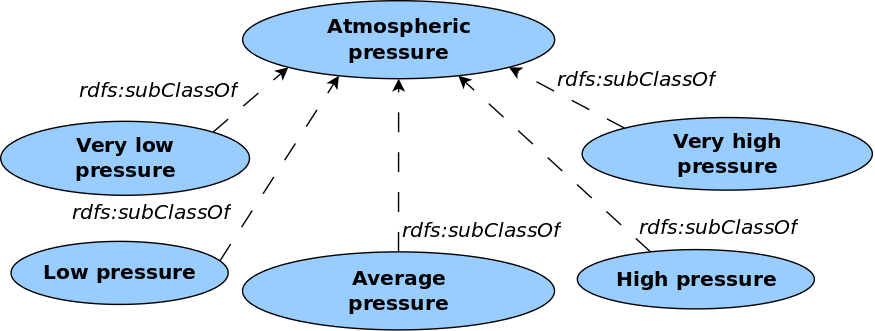
\includegraphics[scale=.3]{figures/diagrams/atmospheric-pressure.png}
\end{center}

\paragraph{Cloud cover}

\begin{center}
  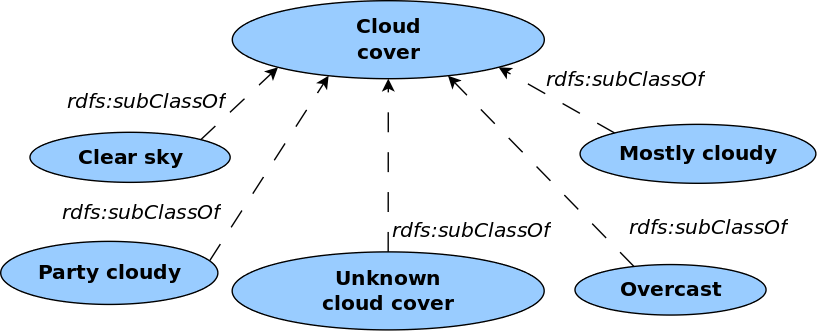
\includegraphics[scale=.3]{figures/diagrams/cloud-cover.png}
\end{center}

\paragraph{Humidity}

\begin{center}
  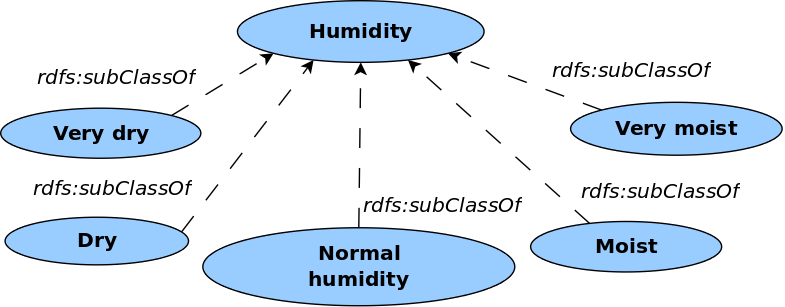
\includegraphics[scale=.3]{figures/diagrams/humidity.png}
\end{center}

\paragraph{Precipitation}

\begin{center}
  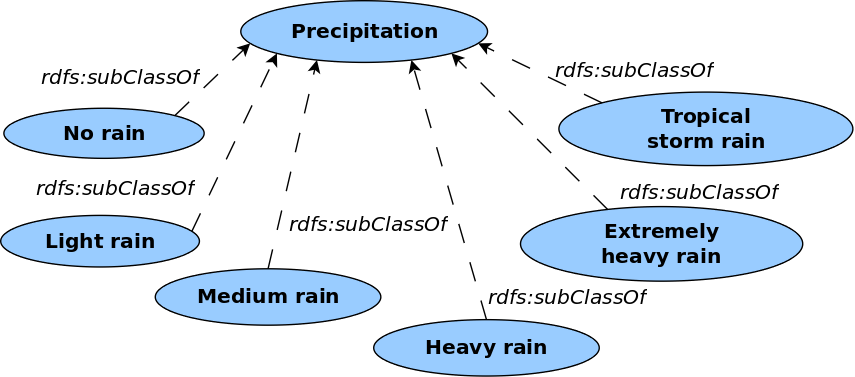
\includegraphics[scale=.3]{figures/diagrams/precipitation.png}
\end{center}

\paragraph{Sun position}

\begin{center}
  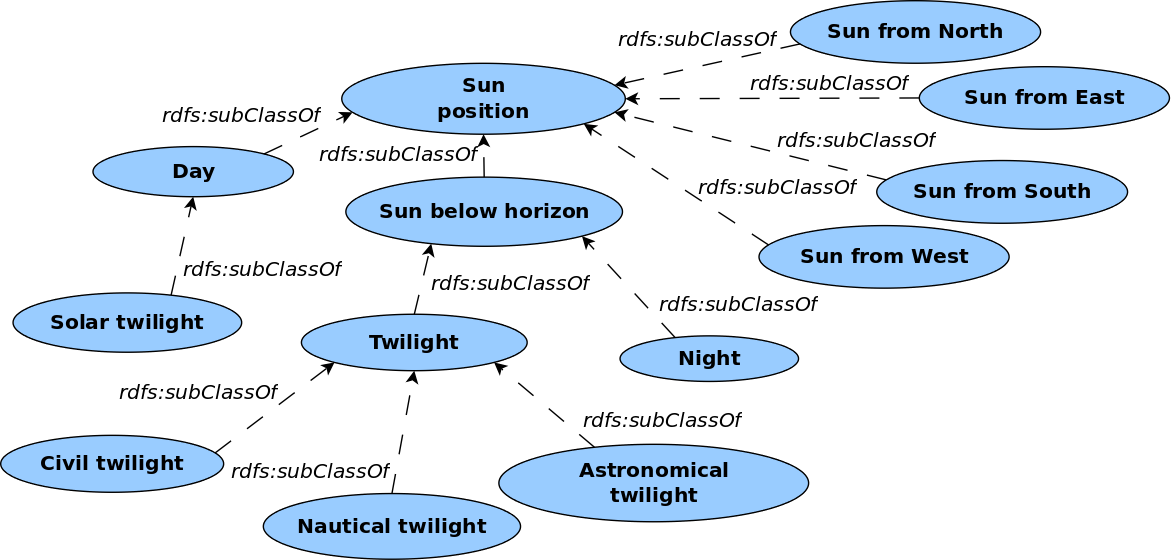
\includegraphics[scale=.3]{figures/diagrams/sun-position.png}
\end{center}

\paragraph{Sun radiation}

\begin{center}
  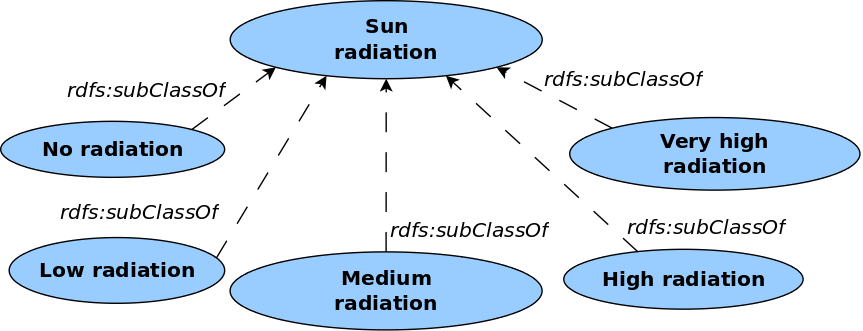
\includegraphics[scale=.3]{figures/diagrams/sun-radiation.png}
\end{center}

\paragraph{Temperature}

\begin{center}
  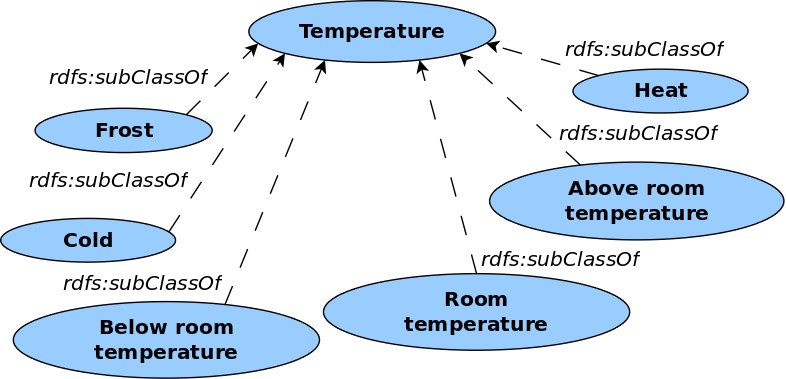
\includegraphics[scale=.3]{figures/diagrams/temperature.png}
\end{center}

\paragraph{Wind}

\begin{center}
  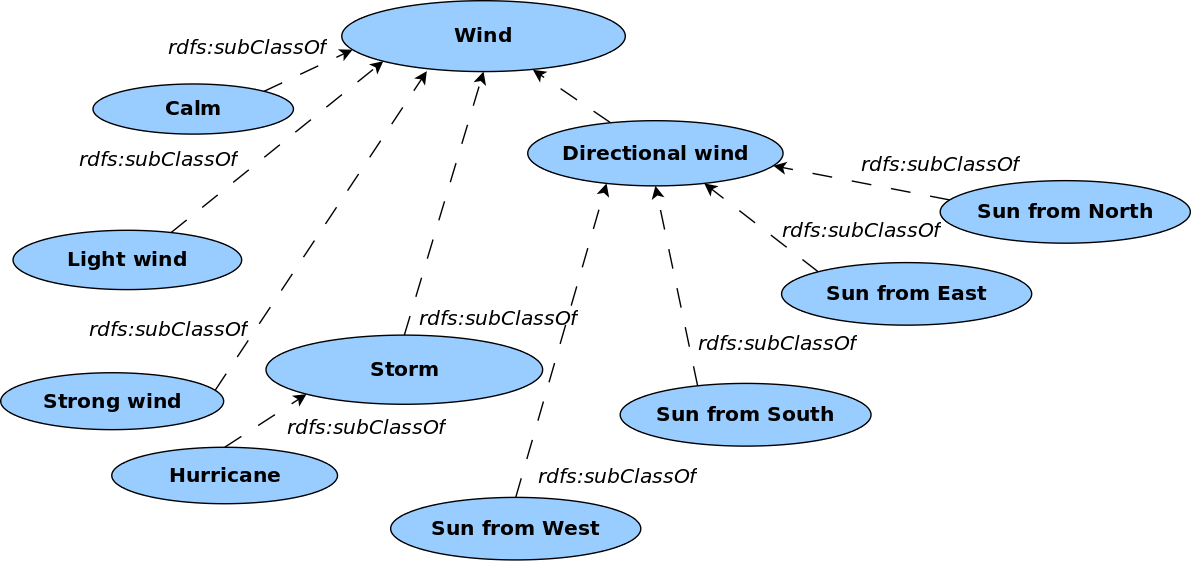
\includegraphics[scale=.3]{figures/diagrams/wind.png}
\end{center}

\subsubsection{Weather report}

There are two main attributes for a \emph{Weather report}: Its \emph{Start date} and its \emph{Source}. A number of sub-concepts is defined in order to reflect different values of these two attributes:

\begin{center}
  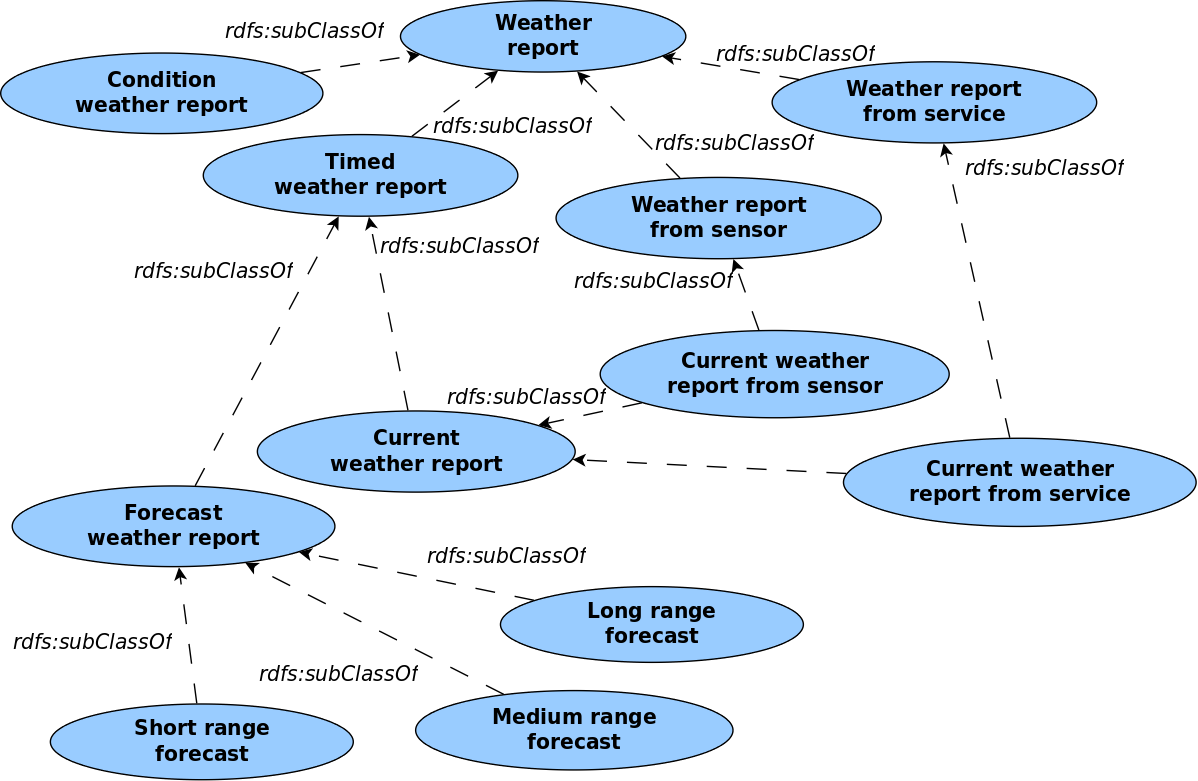
\includegraphics[scale=.3]{figures/diagrams/weather-report.png}
\end{center}

The concepts \emph{Short range forecast}, \emph{Medium range forecast} and \emph{Long range forecast} each do have sub-concepts which have been omitted from the above diagram for clarity. These sub-concepts are:
\begin{itemize}
  \item \emph{Short range forecast}: \emph{Forecast 1 hour weather report}, \emph{Forecast 2 hours weather report} and \emph{Forecast 3 hours weather report} for weather reports describing the weather in one, two and three hours.
  \item \emph{Medium range forecast}: \emph{Forecast 6 hour weather report} and \emph{Forecast 9 hours weather report} for weather reports describing the weather in 6 and 9 hours.
  \item \emph{Long range forecast}: \emph{Forecast 12 hour weather report}, \emph{Forecast 15 hours weather report}, \emph{Forecast 18 hours weather report}, \emph{Forecast 21 hours weather report} and \emph{Forecast 25 hours weather report} for weather reports describing the weather in 12, 15, 18, 21 and 24 hours.
\end{itemize}

\subsubsection{Weather report source}

A \emph{Weather report source} can either be a \emph{Sensor source} or a \emph{Service source}:

\begin{center}
  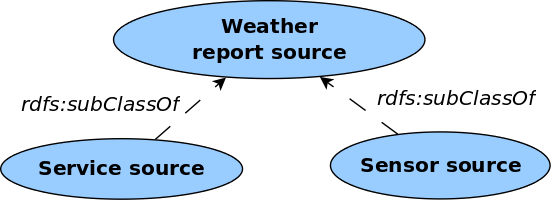
\includegraphics[scale=.3]{figures/diagrams/weather-report-source.png}
\end{center}

\subsubsection{Weather state}

% TODO reformulate this
A \emph{Weather state} collects all \emph{Weather phenomena} for a certain \emph{Weather report}. Because of this, sub-concepts of \emph{Weather state} can be introduced that reflect certain combination of related instances of \emph{Weather phenomenon}:

\begin{center}
  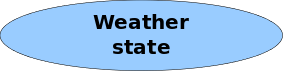
\includegraphics[scale=.3]{figures/diagrams/weather-state.png}
\end{center}

\subsection{Binary relations diagram}
\label{sec:binary_relations_diagram}

The binary relations diagram shows all binary relations between concepts in the ontology in a clear manner:

\begin{center}
  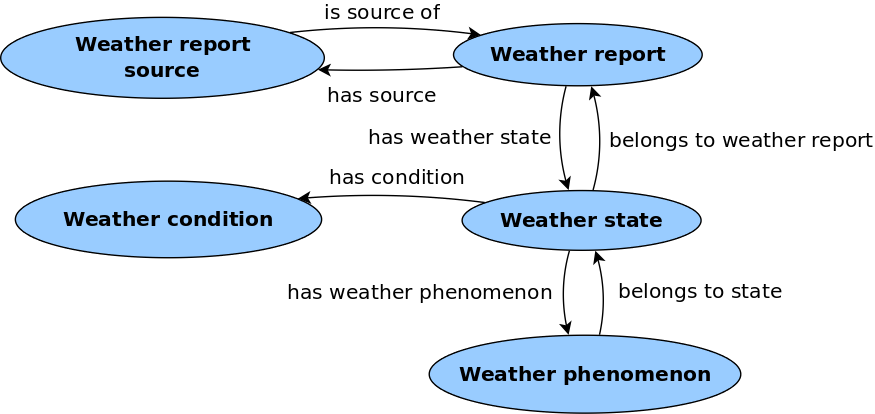
\includegraphics[scale=.3]{figures/diagrams/binary-relations.png}
\end{center}

\subsection{Concept dictionaries}

A concept dictionary lists all concepts together with their names, instances, class attributes, instance attributes and relations. For the sake of clarity, this table is split up into several tables, one for each of the concept-classification trees in section \ref{sec:concept_classification_trees}.

\subsubsection{Weather condition}

\begin{longtable}{|p{0.167\textwidth}|p{0.167\textwidth}|p{0.167\textwidth}|p{0.167\textwidth}|p{0.167\textwidth}|}
  \hline
  \textbf{Name} & \textbf{Instances} & \textbf{Class\newline attributes} & \textbf{Instance\newline attributes} & \textbf{Relations} \\
  \hline\hline
  Weather condition & Cloud\newline Fog\newline Partly cloudy\newline Mostly cloudy\newline Rain\newline Sleet\newline Snow\newline Sun\newline Thunder & - & - & hasCondition \\
  \hline
\end{longtable}

\subsubsection{Weather phenomenon}

% TODO
\begin{longtable}{|p{0.167\textwidth}|p{0.167\textwidth}|p{0.167\textwidth}|p{0.167\textwidth}|p{0.167\textwidth}|}
  \hline
  \textbf{Name} & \textbf{Instances} & \textbf{Class\newline attributes} & \textbf{Instance\newline attributes} & \textbf{Relations} \\
  \hline\hline
  Above room temperature & - & - & - & - \\
  \hline
  Astronomical twilight & - & - & - & - \\
  \hline
  Atmospheric pressure & - & - & - & - \\
  \hline
  Below room temperature & - & - & - & - \\
  \hline
  Calm & - & - & - & - \\
  \hline
  Civil twilight & - & - & - & - \\
  \hline
  Clear sky & - & - & - & - \\
  \hline
  Cloud & - & - & - & - \\
  \hline
  Cloud cover & - & - & - & - \\
  \hline
  Cold & - & - & - & - \\
  \hline
  Day & - & - & - & - \\
  \hline
  Dew point & - & - & - & - \\
  \hline
  Directional wind & - & - & - & - \\
  \hline
  Dry & - & - & - & - \\
  \hline
  East wind & - & - & - & - \\
  \hline
  Extremely heavy rain & - & - & - & - \\
  \hline
  Fog & - & - & - & - \\
  \hline
  Frost & - & - & - & - \\
  \hline
  Heat & - & - & - & - \\
  \hline
  Heavy rain & - & - & - & - \\
  \hline
  High pressure & - & - & - & - \\
  \hline
  High radiation & - & - & - & - \\
  \hline
  Humidity & - & - & - & - \\
  \hline
  Hurricane & - & - & - & - \\
  \hline
  Light rain & - & - & - & - \\
  \hline
  Light wind & - & - & - & - \\
  \hline
  Low pressure & - & - & - & - \\
  \hline
  Low radiation & - & - & - & - \\
  \hline
  Medium radiation & - & - & - & - \\
  \hline
  Medium rain & - & - & - & - \\
  \hline
  Moist & - & - & - & - \\
  \hline
  Mostly cloudy & - & - & - & - \\
  \hline
  Nautical twilight & - & - & - & - \\
  \hline
  Night & - & - & - & - \\
  \hline
  No radiation & - & - & - & - \\
  \hline
  No rain & - & - & - & - \\
  \hline
  Normal humidity & - & - & - & - \\
  \hline
  Normal pressure & - & - & - & - \\
  \hline
  North wind & - & - & - & - \\
  \hline
  Overcast & - & - & - & - \\
  \hline
  Partly cloudy & - & - & - & - \\
  \hline
  Precipitation & - & - & - & - \\
  \hline
  Room temperature & - & - & - & - \\
  \hline
  Solar twilight & - & - & - & - \\
  \hline
  South wind & - & - & - & - \\
  \hline
  Sun from east & - & - & - & - \\
  \hline
  Sun from north & - & - & - & - \\
  \hline
  Sun from south & - & - & - & - \\
  \hline
  Sun from west & - & - & - & - \\
  \hline
  Sun position & - & - & - & - \\
  \hline
  Sun radiation & - & - & - & - \\
  \hline
  Temperature & - & - & - & - \\
  \hline
  Tropical storm rain & - & - & - & - \\
  \hline
  Unknown cloud cover & - & - & - & - \\
  \hline
  Very dry & - & - & - & - \\
  \hline
  Very high pressure & - & - & - & - \\
  \hline
  Very high radiation & - & - & - & - \\
  \hline
  Very low pressure & - & - & - & - \\
  \hline
  Very moist & - & - & - & - \\
  \hline
  Weather phenomenon & - & - & - & - \\
  \hline
  West wind & - & - & - & - \\
  \hline
  Wind & - & - & - & - \\
  \hline
\end{longtable}

\subsubsection{Weather report}

% TODO
\begin{longtable}{|p{0.167\textwidth}|p{0.167\textwidth}|p{0.167\textwidth}|p{0.167\textwidth}|p{0.167\textwidth}|}
  \hline
  \textbf{Name} & \textbf{Instances} & \textbf{Class\newline attributes} & \textbf{Instance\newline attributes} & \textbf{Relations} \\
  \hline\hline
  Altitude & - & - & - & - \\
  \hline
  Current weather report & - & - & - & - \\
  \hline
  Current weather report from sensor & - & - & - & - \\
  \hline
  Current weather report from service & - & - & - & - \\
  \hline
  End time & - & - & - & - \\
  \hline
  Forecast weather report & - & - & - & - \\
  \hline
  Latitude & - & - & - & - \\
  \hline
  Location & - & - & - & - \\
  \hline
  Longitude & - & - & - & - \\
  \hline
  Long range weather report & - & - & - & - \\
  \hline
  Medium range weather report & - & - & - & - \\
  \hline
  Observation time & - & - & - & - \\
  \hline
  Priority & - & - & - & - \\
  \hline
  Short range weather report & - & - & - & - \\
  \hline
  Timed weather report & - & - & - & - \\
  \hline
  Weather report & - & - & - & - \\
  \hline
  Weather report from sensor & - & - & - & - \\
  \hline
  Weather report from service & - & - & - & - \\
  \hline
  & - & - & - & - \\
  \hline
\end{longtable}

\subsubsection{Weather state}

% TODO
\begin{longtable}{|p{0.167\textwidth}|p{0.167\textwidth}|p{0.167\textwidth}|p{0.167\textwidth}|p{0.167\textwidth}|}
  \hline
  \textbf{Name} & \textbf{Instances} & \textbf{Class\newline attributes} & \textbf{Instance\newline attributes} & \textbf{Relations} \\
  \hline\hline
  Condition weather state & - & - & - & - \\
  \hline
  Weather state & - & - & - & - \\
  \hline
  & - & - & - & - \\
  \hline
  & - & - & - & - \\
  \hline
  & - & - & - & - \\
  \hline
  & - & - & - & - \\
  \hline
  & - & - & - & - \\
  \hline
  & - & - & - & - \\
  \hline
  & - & - & - & - \\
  \hline
\end{longtable}

\subsubsection{Weather report source}

% TODO
\begin{longtable}{|p{0.167\textwidth}|p{0.167\textwidth}|p{0.167\textwidth}|p{0.167\textwidth}|p{0.167\textwidth}|}
  \hline
  \textbf{Name} & \textbf{Instances} & \textbf{Class\newline attributes} & \textbf{Instance\newline attributes} & \textbf{Relations} \\
  \hline\hline
  Sensor source & - & - & - & - \\
  \hline
  Service source & - & - & - & - \\
  \hline
  Weather report source & - & - & - & - \\
  \hline
\end{longtable}

\subsection{Binary relations table}

The binary relation table specifies all relations from section \ref{sec:binary_relations_diagram} in detail. This includes the relations' names, their source and target concepts, their maximum source cardinalities and their inverse relations, if any.

\begin{longtable}{|p{0.167\textwidth}|p{0.167\textwidth}|p{0.167\textwidth}|p{0.167\textwidth}|p{0.167\textwidth}|}
  \hline
  \textbf{Name} & \textbf{Source\newline concept} & \textbf{Target\newline concept} & \textbf{Maximum\newline source\newline cardinality} & \textbf{Inverse\newline relation} \\
  \hline\hline
  belongs to state & Weather phenomenon & Weather state & 1 & has weather phenomenon \\
  \hline
  belongs to report & Weather state & Weather report & 1 & has weather state \\
  \hline
  has condition & Weather state & Weather condition & N & - \\
  \hline
  has next weather report & Weather report & Weather report & 1 & has previous weather report \\
  \hline
  has previous weather report & Weather report & Weather report & 1 & has next weather report \\
  \hline
  has source & Weather report & Weather report source & 1 & is source of \\
  \hline
  has weather phenomenon & Weather state & Weather phenomenon & N & belongs to state \\
  \hline
  has weather state & Weather report & Weather state & 1 & belongs to report \\
  \hline
  is source of & Weather report source & Weather report & N & has source \\
  \hline
\end{longtable}

\subsection{Instance attribute tables}
\label{subsec:instance_attribute_tables}

% TODO add these attributes to the Glossary of Terms

% TODO description of what is going on here
% TODO
\begin{longtable}{|p{0.167\textwidth}|p{0.167\textwidth}|p{0.167\textwidth}|p{0.167\textwidth}|p{0.167\textwidth}|}
  \hline
  \textbf{Attribute name} & \textbf{Concept name} & \textbf{Value type} & \textbf{Value range} & \textbf{Cardinality} \\
  \hline\hline
  Altitude & - & - & - & - \\
  \hline
  Cloud altitude & - & - & - & - \\
  \hline
  Cloud cover & - & - & - & - \\
  \hline
  Dew point value & - & - & - & - \\
  \hline
  End time & - & - & - & - \\
  \hline
  Humidity value & - & - & - & - \\
  \hline
  Latitude & - & - & - & - \\
  \hline
  Longitude & - & - & - & - \\
  \hline
  Observation time & - & - & - & - \\
  \hline
  Precipitation intensity & - & - & - & - \\
  \hline
  Precipitation probability & - & - & - & - \\
  \hline
  Pressure value & - & - & - & - \\
  \hline
  Start time & - & - & - & - \\
  \hline
  Sun direction & - & - & - & - \\
  \hline
  Sun elevation angle & - & - & - & - \\
  \hline
  Temperature value & - & - & - & - \\
  \hline
  Wind direction & - & - & - & - \\
  \hline
  Wind speed & - & - & - & - \\
  \hline
\end{longtable}

\subsection{Class attribute tables}

% TODO description of what is going on here
% TODO 
\begin{longtable}{|p{0.167\textwidth}|p{0.167\textwidth}|p{0.167\textwidth}|p{0.167\textwidth}|p{0.167\textwidth}|}
  \hline
  \textbf{Attribute name} & \textbf{Defined concept} & \textbf{Value type} & \textbf{Cardinality} & \textbf{Values} \\
  \hline\hline
  - & - & - & - & - \\
  \hline
\end{longtable}

\subsection{Logical axioms tables}

% TODO sub-concepts of weather state

\subsection{Formula tables}

% TODO sub-concepts of weather state

\subsection{Instance tables}

% TODO description of what is going on here
% TODO
\begin{longtable}{|p{0.2\textwidth}|p{0.2\textwidth}|p{0.2\textwidth}|p{0.2\textwidth}|}
  \hline
  \textbf{Instance name} & \textbf{Concept name} & \textbf{Attribute} & \textbf{Values} \\
  \hline\hline
  Cloud & Weather condition & - & - \\
  \hline
  Fog & Weather condition & - & - \\
  \hline
  Partly cloudy & Weather condition & - & - \\
  \hline
  Mostly cloudy & Weather condition & - & - \\
  \hline
  Rain & Weather condition & - & - \\
  \hline
  Sleet & Weather condition & - & - \\
  \hline
  Snow & Weather condition & - & - \\
  \hline
  Sun & Weather condition & - & - \\
  \hline
  Thunder & Weather condition & - & - \\
  \hline
\end{longtable}

\section{Integration}
\label{sec:integration}

One of the goals of the \thinkhomeweather ontology is to keep an eye on existing ontologies to be re-used. While analyzing the problem domain, it quickly became clear that there are four areas where already existing ontologies could be reused: Location data, measuremenr units, date/time specifications and weather concepts. Chapter \label{ch:existing_work} already shed some light on existing ontologies around the domain of weather data. In this section, the ontologies being short-listed for reuse within \thinkhomeweather are summarized.

% TODO reference: website, WGS84
For location data, the W3C Semantic Web Interest Group offers a \emph{Basic Geo (WGS84 lat/long) Vocabulary}. It introduces a concept called \emph{Spatial thing} that can have \emph{latitude}, \emph{longitude} and \emph{altitude} according to the WGS 84 geodetic reference system. However, the vocabulary contains some data properties that are incorrectly defined as annotation property. This shortcoming needs to be overriden in any ontology that uses this vocabulary.

% TODO reference SWEET
NASA's SWEET ontology offers a wide range of concepts, attributes and individuals for environmental and atmospherical phenomena, including all units that may be used within a weather data ontology. SWEET is designed in a highly modular manner. Units can be found in a single OWL file. However, importing one of SWEET's OWL files into an ontology entails the import of a large number of other OWL files. As this makes any simple ontology using SWEET hard to handle, reusing SWEET is not an option.

Besides SWEET, there is no appropriate ontology containing weather concepts that would make sense to be reused within \thinkhomeweather ontology. Hence, \thinkhomeweather defines its own weather concepts.

% TODO reference: http://forge.morfeo-project.org/wiki_en/index.php/Units_of_measurement_ontology
% TODO reference: http://idi.fundacionctic.org/muo/muo-vocab.html
The \emph{Measurement Units Ontology} is a simple and light-weight approach to enrich measurement values with appropriate units. Some of the most important units are pre-defined, all others can easily be added. The \emph{Measurement Units Ontology} (MUO) is still work in progress. However, it is not expected that it might change heavily in the future. Everything that will be reused by other ontologies will remain unchanged. Hence, MUO can be imported into any ontology without problems.

% TODO reference W3C consortium
% TODO reference W3C working draft definition
% TODO reference http://www.w3.org/TR/owl-time/
For specifying temporal properties, the W3C consortium offers a working draft of \emph{OWL-Time}, a \emph{Time Ontology in OWL}. It defines the concept called \emph{TemporalEntity} that can either be an \emph{Instant} or an \emph{Interval}. Using appropriate attributes, the properties of a \emph{TemporalEntity} are specified. Although \emph{OWL-Time} is in the state of a working draft since September 2006, the main concepts and attributes that will be reused by other ontologies are expected not to change in any way.

% TODO mention meta-ontology

Section \ref{sec:implementation} describes the reuse of the aforementioned ontologies within the \thinkhomeweather ontology in detail.

\section{Implementation}
\label{sec:implementation}

After exhaustive analysis and structurization in the previous sections, the step of implementing the ontology has become a straight-forward task.

% TODO reference OWL, Protege, Pellet
% TODO \emph{} for names
The \thinkhomeweather ontology is implemented in OWL using Protege 4.1 together with the Pellet OWL 2 Reasoner. Pellet includes Pellint, an ontology performance tool that uses a set of patterns to find possible performance problems in an OWL ontology. Pellint has been used for locating problems and led to a few improvements boosting reasoning performance.

To ensure that the reasoning of all sub-concepts of \emph{Weather phenomenon}, \emph{Weather state} and \emph{Weather report} works correctly, a JUnit is used. Every test case loads the \thinkhomeweather ontology using the \emph{Jena framework}, adds appropriate individuals and checks using the \emph{Pellet reasoner} if reasoning is performed in the desired manner.

\subsection{Imported ontologies}

During the implementation step, the ontologies listed in section \ref{sec:integration} need to be imported and integrated. Their use implies the application of certain patterns required by the ontologies.

% TODO reference OWL-Time
\emph{OWL-Time} defines the concept \emph{TemporalEntity} and its sub-concepts \emph{Instant} and \emph{Interval}. Although \emph{Start time} and \emph{End time} of a \emph{Weather report} are actually \emph{Instant}s, these times are specified using \emph{Interval}s. The duration of such an interval represents the duration between the \emph{Observation time} of the \emph{Weather report} and the time that is to be expressed. This results in the structure shown in figure . % TODO reference figure
The duration is rounded to full hours. Hence, there are simple rules for defining concepts for a \emph{Weather report} for forecasts in an arbitrary number of hours.

% TODO figure

The \emph{Observation time} of a \emph{Weather report} is specified using an \emph{Instant} as defined by \emph{OWL-time}. See figure ... for the resulting structure. % TODO reference figure

% TODO figure

The \emph{Time Zone Ontology} that comes with \emph{OWL-Time} is not used by \thinkhomeweather. All times must be given in UTC.

% TODO reference unit ontology
All instances of \emph{Weather phenomenon} have one or more attributes specifying details about the weather element that is being represented (refer to section \label{subsec:instance_attribute_tables} for details about these attributes). Each of these attributes assigns a numerical value to the \emph{Weather phenomenon}. To avoid confusion by the use of different units for one attribute (e.g. $^\circ$F and $^\circ$C for the \emph{Temperature value}), concepts, attributes and instances from the \emph{Measurement Units Ontology} (MUO) are re-used to add unit information. MUO forces the use of a certain pattern that is shown in figure . % TODO reference figure

% TODO reference WGS-84
The \emph{Basic Geo (WGS84 lat/long) Vocabulary} by the \emph{W3C Semantic Web Interest Group} defines the concept \emph{Point} together with the attributes \emph{lat} (latitude), \emph{long} (longitude) and \emph{alt} (altitude). Furthermore, the attribute \emph{location} offers the possibility of connecting a \emph{Point} to any instance of some concept. See figure ... for the structure that results from this. % TODO reference figure

\begin{center}
  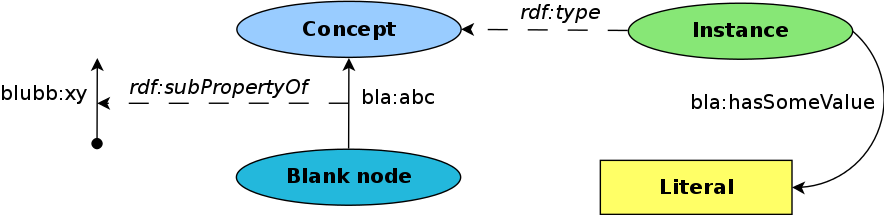
\includegraphics[width=\textwidth]{figures/diagrams/template.png}
\end{center}

% TODO figure

% TODO document completed ontology thoroughly
% TODO diagrams for parts of the ontology
\subsection{Naming conventions}

During the implementation of the \thinkhomeweather ontology, it was necessary to define strict naming conventions for concepts, individuals and attributes; some of these conventions have already been applied to previous steps of developing the ontology:

\begin{itemize}
  \item All concepts, instances and attributes share one namespace, regardless of capitalization; e.g. there is no pair of a concept and an instance that shares the same name. There is also no pair of a concept and an instance which names only differ in their capitalization.
  \item Only upper case and lower case letters from A to Z, numbers from 0 to 9, underscores (\texttt{\_}) and dashes (\texttt{-}) may occur in the name of a concept, an instance or an attribute. Hence, all names match the regular expression \texttt{\^{}[A-Za-z0-9\textbackslash -\_]\$}.
  \item Names built from more than one word are written in \emph{Camel case}, e.g. \emph{Weather phenomenon} becomes \emph{WeatherPhenomenon} and \emph{is source of} becomes \emph{isSourceOf}. % TODO reference to camel case definition?
  \item Concept names start with a capital letter and only appear in singular. There is no concept name \emph{Weather phenomena}, only \emph{WeatherPhenomenon}.
  \item Attribute names start with a lower-case letter. Attribute names are always built from more than one word and the first word must be a verb; see \emph{isSourceOf} or \emph{hasWeatherCondition}.
\end{itemize}


\section{Evaluation}
\label{ch:ontology_evaluation}

% TODO compare existing ontology with specification and competence questions

\section{Fetching data}

% TODO describe fetching weather data from yr.no
% TODO describe algorithms for calculation of the position of the sun
% TODO perhaps split into two categories (one for weather data and one for the sun's position according to one of the two available algorithms, see SunPositionCalculator's source code

% TODO reference section/subsection instead of chapter?
As discussed in chapter \ref{ch:weather_data}, among all internet services that have been analyzed, \emph{yr.no} is the API that best fits the requirements for the \thinkhomeweather ontology. This section covers acquisition of weather data from that service in detail.

% TODO reference Jena framework
A Java application called \emph{WeatherReader} was developed. It processes weather data in two steps:

\begin{itemize}
  \item In the first step, the application uses the API of \emph{yr.no} to fetch weather data(see \ref{subsec:weather_data_yr_no}). Additionally, sun position data is calculated (see \ref{subsec:sun_position}). Data is stored in a specially built domain model. % See figure \ref{...} for the UML class diagram of the domain model used by \emph{WeatherReader}.
  \item The second step, individuals are created based on the weather data that has been previously acquired. This results in a new ontology based on the \thinkhomeweather ontology enriched by appropriate individuals.
\end{itemize}

% TODO UML class diagram of the domain model used by \emph{WeatherReader}.

Using a configuration file, \emph{WeatherReader} is fully customizable regarding OWL files and location.

\subsection{Weather data}
\label{subsec:weather_data_yr_no}

% TODO fix overfull hboxes in this subsection

% TODO reference http://api.yr.no/weatherapi/locationforecast/1.8/documentation
For an arbitrary request, one must specify latitude and logitude (in degrees, nothern latitudes and eastern longitudes are represented by positive values). Additionally, the altitude above sea level (in metres) may be specified for locations outside Norway. Based on this input data, a URL of the format

% TODO move this definition to some other position
% TODO improve formatting of lstlisting environments
\lstset{frame=trbl}
\begin{lstlisting}
http://api.yr.no/weatherapi/locationforecast/1.8/?lat=<latitude>;lon=<longtude>
\end{lstlisting}

or

\begin{lstlisting}
http://api.yr.no/weatherapi/locationforecast/1.8/?lat=<latitude>;lon=<longtude>;msl=<altitude>
\end{lstlisting}

is built, e.g.

\begin{lstlisting}
http://api.yr.no/weatherapi/locationforecast/1.8/?lat=48.21;lon=16.37;msl=171
\end{lstlisting}

% TODO explicitly name lat, lon, msl for Vienna
for the city of Vienna, Austria. A GET request to this URL returns an XML document conforming to the XML Schema definition that can be found
% TODO reference http://api.yr.no/weatherapi/locationforecast/1.8/schema
online.

The structure of the XML document is as follows (attributes are omitted for better readability):

\begin{lstlisting}
<weatherdata>
	<meta>
		<model />
	</meta>
	<product>
		/* ... */
	</product>
</weatherdata>
\end{lstlisting}

The attributes of the <model> element specify when the forecast has been created, when it will be updated for the next time and what date and time of the first and the last forecast returned are.

There is an arbitrary number of <time> elements that are children of the <product> element. Every <time> element represents the weather forecast for a certain period of time. Each <time> element has a <location> element that has a child element for each weather property.

This is a typical <time> element:

\begin{lstlisting}
<time datatype="forecast" from="2011-10-17T09:00:00Z" to="2011-10-17T09:00:00Z">
	<location altitude="171" latitude="48.2100" longitude="16.3700">
		<temperature id="TTT" unit="celcius" value="8.5" />
		<windDirection id="dd" deg="140.3" name="SE" />
		<windSpeed id="ff" mps="4.5" beaufort="3" name="Lett bris" />
		<humidity value="45.1" unit="percent" />
		<pressure id="pr" unit="hPa" value="1027.6" />
		<cloudiness id="NN" percent="0.0" />
		<fog id="FOG" percent="0.0" />
		<lowClouds id="LOW" percent="0.0" />
		<mediumClouds id="MEDIUM" percent="0.0" />
		<highClouds id="HIGH" percent="0.0" />
	</location>
</time>
\end{lstlisting}

% TODO format names?
% TODO group names (e.g. for temperature, humidity, clouds, ...)?
The names of the elements that are allowed to be children of the <location> element are: groundCover, pressure, maximumPrecipitation, highestTemperature, lowestTemperature, precipitation, fog, cloudiness, lowClouds, mediumClouds, highClouds, temperature, dewpointTemperature, minTemperatureDay, minTemperatureNight, maxTemperatureDay, maxTemperatureNight, uv, tidalwater, currentDirection, maxWaveHeight, surfaceTemperature, waveDirection, wavePeriod, waveHeight, humidity, bias, numberofobservations, meanabsoluteerror, score, windDirection, windSpeed, maxWindSpeed, stateOfTheSea, snowDepth, weather, symbol, forest-fire, windProbability, temperatureProbability and symbolProbability.

None of the child elements are required. However, for most places of the world, the XML document contains <location> elements having two different sets of child elements:

\begin{itemize}
  \item Some <location> elements have the child elements temperature, windDirection, windSpeed, humidity, pressure, cloudiness, fog, lowClouds, mediumClouds and highClouds (as shown above). The values of the attributes from and to of the enclosing <time> element are equal.
  \item Some <location> elements have the child elements precipitation and symbol; the values of the attributes from and to of the enclosing <time> element differ by three to six hours; such an element looks like this:
\end{itemize}

\begin{lstlisting}
<time datatype="forecast" from="2011-10-17T03:00:00Z" to="2011-10-17T09:00:00Z">
	<location altitude="171" latitude="48.2100" longitude="16.3700">
		<precipitation unit="mm" value="0.0" />
		<symbol id="SUN" number="1" />
	</location>
</time>
\end{lstlisting}

The content of the XML document covers a period of nine days, starting at the current day.

\subsection{Position of the sun}
\label{subsec:sun_position}

% TODO reference http://api.yr.no/weatherapi/sunrise/1.0/documentation
Besides location-based weather data, \emph{yr.no} offers an interface for retrieving sunrise and sunset data. Given a position in latitude and longitude together with a date, the times of rise and set of sun and moon will be provided. The angle of the sun at solar noon is also given.

However, these data are inappropriate for use within the \thinkhomeweather ontology as every \emph{Weather state} may be linked to an instance of \emph{Sun position}. \emph{Sun position} has two attributes which are \emph{has sun elevation angle} and \emph{has sun direction} that specify the sun's position. However, none of these values can be calculated from the data provided by \emph{yr.no}.

% TODO reference PSA algorithm: http://www.sciencedirect.com/science/article/pii/S0038092X00001560
% TODO reference SPA algorithm:  Reda, I.; Andreas, A. (2003): Solar Position Algorithm for Solar Radiation Applications. NREL Report No. TP-560-34302, Revised January 2008
% TODO reference http://www.psa.es/sdg/sunpos.htm - terms of use?
% TODO give informations about precision of PSA and SPA
There are some algorithms for calculating the sun's position at a certain location given by latitude and longitude at a certain time. The \emph{SPA algorithm} is a rather complicated algorithm, but it yields results with uncertainities of less than 0.0003 degrees. A simpler algorithm is the \emph{PSA algorithm}. Its results differ from the actual values more than the ones calculated by the \emph{SPA algorithm}. As approximate values for the sun's position are appropriate for use in the \thinkhomeweather ontology, the \emph{PSA algorithm} is suitable for use by the \emph{WeatherReader} application. There are even complete implementations of PSA in C++ that can easily be ported to Java.
